%-------------------------------------------------------------------------------
%-------------------------------------------------------------------------------
%-------------------------------------------------------------------------------
\chapter{Images}
%-------------------------------------------------------------------------------
%-------------------------------------------------------------------------------
\thispagestyle{empty}
%-------------------------------------------------------------------------------
%-------------------------------------------------------------------------------
%--------------------------------------------------------------------------
%--------------------------------------------------------------------------
%--------------------------------------------------------------------------
\section{Présentation}
%--------------------------------------------------------------------------
%--------------------------------------------------------------------------
\subsection{Introduction}
%--------------------------------------------------------------------------
Une image est codée dans un ordinateur sous la forme de petits carrés appelés \type{pixel}s\footnote{{\bf pic}ture {\bf el}ements}. Ces éléments sont rassemblés dans une matrice dont les lignes et les colonnes correspondent aux positions dans l'image.

Pour commencer de façon basique, on peut coder avec des 0 (pas de lumière) et des 1  (de la lumière). 
Voici une première image simple :

\begin{verbatim}
image1 = np.array([[1, 1, 1, 1, 1, 1, 1, 1, 1, 1, 1, 1], 
                   [1, 0, 1, 0, 1, 0, 1, 0, 1, 0, 0, 1], 
                   [1, 0, 1, 1, 1, 0, 1, 0, 1, 0, 1, 1], 
                   [1, 0, 1, 0, 1, 0, 1, 0, 1, 0, 1, 1], 
                   [1, 0, 1, 0, 1, 0, 1, 0, 1, 0, 0, 1], 
                   [1, 0, 1, 0, 1, 0, 1, 0, 1, 0, 1, 1], 
                   [1, 0, 1, 0, 1, 0, 1, 0, 1, 0, 1, 1], 
                   [1, 0, 1, 0, 1, 0, 1, 0, 1, 0, 0, 1], 
                   [1, 1, 1, 1, 1, 1, 1, 1, 1, 1, 1, 1]])
\end{verbatim}

On remarquera qu'on a utilisé une matrice, c'est-à-dire une liste de listes, convertie en matrice \type{numpy} avec \type{np.array} : les calculs seront plus rapides pour les grandes tailles et il est plus facile de sélectionner des morceaux.

On devra donc auparavant charger les bibliothèques
\begin{lstlisting}
import numpy as np
import matplotlib.pyplot as plt
\end{lstlisting}

Pour voir ce que représente cette image on peut colorier les 0 en noir.

On peut aussi la faire afficher : 
\begin{lstlisting}
plt.imshow(image1)
plt.show()
\end{lstlisting}
Ce n'est pas vraiment ce que l'on attendait car Python choisit une échelle de couleurs par défaut qui n'est pas une échelle de gris.
  
On peut voir cette échelle en tapant \type{plt.colorbar()}.
  
Si on veut simplement une échelle de gris, on peut le spécifier par la commande \type{plt.gray()}.

On peut aussi changer l'échelle des couleurs avec le paramètre \type{cmap} (pour Color MAP)
  
  \type{plt.imshow(image1, cmap='gray')}
  
On peut voir les différentes échelles de couleur à l'adresse
  
\begin{verbatim}
  http://matplotlib.org/examples/color/colormaps_reference.html
\end{verbatim}
%--------------------------------------------------------------------------
\subsection{Niveaux}
%--------------------------------------------------------------------------
On a vu qu'il y avait une échelle, on peut choisir des valeurs intermédiaires. 

L'échelle s'adapte : l'intervalle des valeurs sera toujours $[a;b]$ où $a$ est le minimum des valeurs de la matrice et $b$ le maximum.

\begin{lstlisting}
image2 = np.zeros((100,100))
for i in range(100):
    for j in range(100):
        x = (i-50)/20
        y = (j-50)/20
        image2[i,j] = np.sin(x*x+y*y)

plt.imshow(image2)
plt.show()
\end{lstlisting}

Si on affiche l'échelle des couleurs on voit que les valeurs utilisées vont de $-1$ à 1.

L'image présente un effet de carrelage, on voit les pixels. On peut estomper les différences en ajoutant une interpolation :
\begin{lstlisting}
plt.imshow(image2, interpolation = 'bilinear')
\end{lstlisting}
%--------------------------------------------------------------------------
\subsection{Photos monochromes}
%--------------------------------------------------------------------------
Ce qui précède utilise la représentation des matrices pour illustrer des données : la valeur atteinte par une fonction de deux variables (les coordonnées) est visualisée par sa couleur dans une échelle.

On peut aussi penser ces valeurs comme la luminosité d'un point et considérer une matrice comme une image, par exemple une photo en noir-et-blanc.

Dans \type{scipy.misc} on peut trouverun exemple de photo. 

\begin{lstlisting}
from scipy.misc import ascent

image4 = ascent()
plt.gray()
plt.imshow(image4)
plt.show()
\end{lstlisting}

\type{matplotlib} permet de lire des images en format \type{png} et les transforme en matrice \type{numpy}.

Le dossier {\ss public} devrait contenir une photo du Taj-Mahal.

\begin{lstlisting}
imgage5 = plt.imread('chemin/vers/le/fichier/taj-NB.png')
plt.gray()
plt.imshow(imgage5)
plt.show()
\end{lstlisting}


Nous allons dans ce TP modifier une image.

Comme il est souhaitable de garder inchangée l'image originale on devra

\begin{itemize}
\item soit copier l'image, \type{img = np.copy(image)}
\item soit créer une image de zéros de même taille
\begin{lstlisting}
p,q = np.shape(image)
img = np.zeros((p,q))
\end{lstlisting}
Il existe une astuce pour les matrices \type{numpy} pour ce dernier cas : \type{img = 0*image}.
\end{itemize}
%--------------------------------------------------------------------------
%--------------------------------------------------------------------------
\section{Modification de l'échelle}
%--------------------------------------------------------------------------
%--------------------------------------------------------------------------

La première action possible sur une image est de modifier globalement la valeur des pixels.

Nous avons vu que \type{matplotlib} s'adaptait à l'intervalle des valeurs : il détermine les minimum et maximum et distribue la coloration entre ces extrêmes.

Cependant, par cohérence avec les images en couleur, nous allons nous restreindre à une échelle de valeur entre 0 et 1.

On définit donc \type{image1 = ascent()/255} car l'échelle initiale va de 0 à 255.

Le principe général sera de déterminer une fonction de $[0;1]$ dans lui même que l'on appliquera à tous les pixels.

\begin{center}

Exercice 1 : 
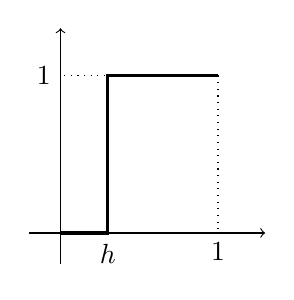
\begin{tikzpicture}[scale=2]
\draw[->] (-0.2,0) -- (1.3,0);
\draw[->] (0,-0.2) -- (0,1.3);
\draw[very thick] (0,0) -- (0.3,0) node[below]{$h$} 
                   -- (0.3,1) -- (1,1);
\draw[dotted] (1,1) -- (1,0) node[below]{1};
\draw[dotted] (1,1) -- (0,1) node[left]{1};
\end{tikzpicture}
\hskip 2cm
Exercice 2 : 
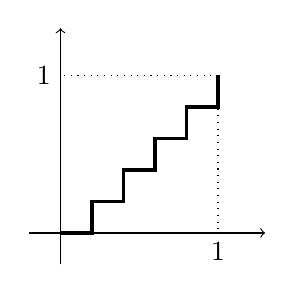
\begin{tikzpicture}[scale=2]
\draw[->] (-0.2,0) -- (1.3,0);
\draw[->] (0,-0.2) -- (0,1.3);
\draw[very thick] (0,0) -- (0.2,0) -- (0.2,0.2) 
                   -- (0.4,0.2) -- (0.4,0.4)
                   -- (0.6,0.4) -- (0.6,0.6)
                   -- (0.8,0.6) -- (0.8,0.8)
                   -- (1.0,0.8) -- (1.0,1.0);
\draw[dotted] (1,1) -- (1,0) node[below]{1};
\draw[dotted] (1,1) -- (0,1) node[left]{1};
\end{tikzpicture}
\end{center}

%--------------------------------------------------------------------------
\begin{Exercise}[title=Image en noir et blanc]\it Écrire une fonction \type{seuil(x,h)} qui reçoit deux réels $x$ et $h$ et qui renvoie 0 dans la cas $x<h$ et 1 sinon.
En déduire une fonction \type{seuil\_image(image,h)} qui reçoit une image sous la forme d'une matrice \type{numpy} et un réel $h\in [0;1]$ et qui renvoie une nouvelle image dont les éléments sont les images par \type{seuil(x,h)} pour tous les pixels $x$ de l'image initiale.
\end{Exercise}
%--------------------------------------------------------------------------
\begin{Answer}
\begin{lstlisting}
def seuil(h,x):
    if x < h:
        return 0
    else:
        return 1
        
def seuil_image(image,h):
    img = np.copy(image)
    a, b = np.shape(img)
    for i in range(a):
        for j in range(b):
            img[i,j] = seuil(h,img[i,j])
    return img
\end{lstlisting}
\end{Answer}
%--------------------------------------------------------------------------

\medskip

On peut généraliser en calculant plusieurs valeurs de seuil : on obtient un effet de sérigraphie.

La fonction $x \mapsto \frac 1n \lfloor nx\rfloor$ ne donnera que les valeurs $0$, $\frac 1n$, $\frac 2n$, \dots, $\frac {n-1}n$, $1$
%--------------------------------------------------------------------------
\begin{Exercise}[title=Image posterisée]\it Écrire une fonction \type{poster(image,k)} qui reçoit une image et un entier $k$ et qui renvoie une nouvelle image dont les éléments ne prennent que les valeurs de la forme $\frac jk$.

On pourra utiliser \type{cmap = "gist\_rainbow"}.
\end{Exercise}
%--------------------------------------------------------------------------
\begin{Answer}
\begin{lstlisting}
def discretiser(x,k):
    return np.floor(k*x)/k
    
def poster(image,k):
    img = np.copy(image)
    a, b = np.shape(img)
    for i in range(a):
        for j in range(b):
            img[i,j] = discretiser(img[i,j],k)
    return img
\end{lstlisting}
On peut appliquer la fonction directement à un tableau \type{numpy}.

\begin{lstlisting}
def poster(image,k):
    return discretiser(image,k)
\end{lstlisting}

Cela n'a pas été fait dans la question précédente car la fonction avec des tests ne peut pas être distribuée sur une matrice. On peut la transformer pour que cela soit possible 

\begin{lstlisting}
seuil_img = np.vectorize(seuil_image)
\end{lstlisting}

On applique ensuite  la nouvelle fonction \type{seuil\_img}.


\end{Answer}
%--------------------------------------------------------------------------
\medskip

On peut aussi modifier les valeurs en les orientant vers le blanc ou le noir. Il suffit de trouver une fonction de $[0;1]$ dans lui même qui vérifie $f(x) \ge x$ pour donner plus de luminosité ou $f(x) \le x$ pour assombrir.

Les fonctions $x \mapsto x^a$ sont des bons candidats : $a>1$ assombrit, $a<1$ éclaircit.
%--------------------------------------------------------------------------
\begin{Exercise}[title=Luminosité,label=ex:lum]\it Écrire une fonction \type{luminosite(image,a)} qui reçoit une image et un réel $a>0$ et qui renvoie une nouvelle image transformée par $x\mapsto x^a$.
\end{Exercise}
%--------------------------------------------------------------------------
\begin{Answer} 

\begin{lstlisting}
def luminosite(image, a):
    return image**a
\end{lstlisting}
\end{Answer}
%--------------------------------------------------------------------------
\medskip

Plutôt que déplacer la luminosité on peut modifier la différentiation entre le noir et le blanc : le contraste.
 Augmenter le contraste consiste à diminuer les petites valeurs et augmenter les grandes.

Les fonctions que l'on recherche auront un graphe qui ressemble aux graphes suivant

\begin{center}
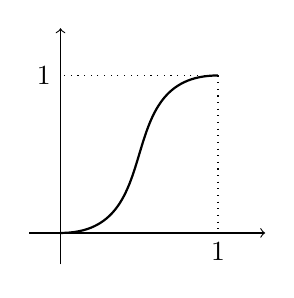
\begin{tikzpicture}[scale=2]
\draw[->] (-0.2,0) -- (1.3,0);
\draw[->] (0,-0.2) -- (0,1.3);
\draw[thick] (0,0) .. controls (0.7,0) and (0.3,1) ..(1,1);
\draw[dotted] (1,1) -- (1,0) node[below]{1};
\draw[dotted] (1,1) -- (0,1) node[left]{1};
\end{tikzpicture}
\hskip 2cm
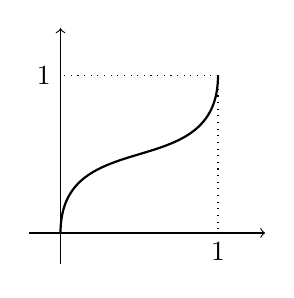
\begin{tikzpicture}[scale=2]
\draw[->] (-0.2,0) -- (1.3,0);
\draw[->] (0,-0.2) -- (0,1.3);
\draw[thick] (0,0) .. controls (0,0.7) and (1,0.3) ..(1,1);
\draw[dotted] (1,1) -- (1,0) node[below]{1};
\draw[dotted] (1,1) -- (0,1) node[left]{1};
\end{tikzpicture}
\end{center}

Ces fonctions peuvent être obtenue à l'aide de \type{np.sin} ou \type{np.arcsin}. 

Par exemple la première fonction est $y = \frac 12 \left(1+\sin\left(\pi\left(x-\frac 12\right)\right)\right)$.
%--------------------------------------------------------------------------
\begin{Exercise}[title=Contraste]\it Écrire des fonctions \type{contrastePlus(image)} et \type{contrasteMoins(image)} qui reçoivent une image et qui renvoient une nouvelle image dont le contraste a été augmenté ou diminué.
\end{Exercise}
%--------------------------------------------------------------------------
\begin{Answer} 
\begin{lstlisting}
def contrastePlus(image):
    return (np.sin((2*image-1)*np.pi/2)+1)/2

def contrasteMoins(image):
    return np.arcsin(2*image-1)/np.pi+1/2
\end{lstlisting}
\end{Answer}
%--------------------------------------------------------------------------
%--------------------------------------------------------------------------
\section{Modifications locales}
%--------------------------------------------------------------------------
%--------------------------------------------------------------------------
Dans cette partie nous allons modifier les images de manière locale : un point sera modifié en fonction de son environnement.

L'outil utilisé est la {\bf convolution} : on veut modifier une image représentée par une matrice $M$ de taille $n\times m$. On se donne une matrice $c$ de taille $(2p+1)\times(2p+1)$ et on remplace chaque pixel $M_{i,j}$ par \[ M'_{i,j} = \sum_{k=0}^{2p}\sum_{l=0}^{2p}M_{i-p+k,j-p+l}c_{k,l}\] pour $p\le i < n-p$ et $p \le j < m-p$. On a utilisé des indices commençant par 0.

On pourra laisser les $p$ lignes ou colonnes des bords avec une valeur nulle.
%--------------------------------------------------------------------------
\begin{Exercise}[title=Convolution]\it Écrire une fonctions \type{convoler(image,noyau)} qui reçoit une image et une matrice de coefficients et qui renvoie une nouvelle image dont les coefficients sont calculés par la formule ci-dessus.
\end{Exercise}
%--------------------------------------------------------------------------
\begin{Answer} 
La version normale demande de parcourir chaque point en lui faisant calculer un produit de deux matrices, cela donne 4 boucles {\bf for} imbriquées.

\newpage

\begin{lstlisting}
def convoler(image,noyau):
    m,n = np.shape(image)
    p,q = np.shape(noyau) 
    img = np.zeros((m,n))
    p1 = (p-1)//2
    for i in range (p1,m-p1): 
        for j in range(p1,n-p1):
            for k in range(p):
                for l in range(p):
                    img[i,j] = img[i,j]
                              +noyau[k,l]*image[i-p1+k,j-p1+l]
    return img
\end{lstlisting}

Cette solution sera assez lente : on peut l'améliorer en sommant par blocs ; on découpe un rectangle dans la matrice autour de la partie centrale, on le multiplie par le coefficient du noyau et on ajoute.
\begin{lstlisting}
def convoler(image,noyau):
    m,n = np.shape(image)
    p,q = np.shape(noyau)
    img = np.zeros((m,n))
    p1 = (p-1)//2
    for i in range(p):
        for j in range(p):
            img[p1:-p1,p1:-p1] += noyau[i,j]
                                 *image[i:m-p+1+i,j:n-q+1+j]
    return img
\end{lstlisting}
Le gain de vitesse est net : on passe dans les exemples de 13 secondes à 0,04 secondes.
\end{Answer}
%--------------------------------------------------------------------------
\begin{Exercise}[title=Floutage]\it Pour calculer une image floutée on peut déterminer la convolution avec une matrice 
$5x5$ dont les coefficients sont $\frac 1{25}$.
\end{Exercise}
%--------------------------------------------------------------------------
\begin{Answer} 
\begin{lstlisting}
flou = np.ones((5,5))/25
image6= convoler(image,flou)
\end{lstlisting}
\end{Answer}
%--------------------------------------------------------------------------
\begin{Exercise}[title=Netteté]\it On peut, inversement, augmenter le "piqué" de la photo en augmentant le contraste local. 

On pourra utiliser la matrice $\begin{pmatrix} 0&-1&0\\ -1&5&-1\\ 0&-1&0\\ \end{pmatrix}$.

Cependant il y a des petits défauts dans la photo qui donnent de grandes valeurs indésirables au résultat. On pourra tronquer les valeurs en remplaçant les négatifs par 0 et les valeurs supérieures à 1 par 1. 
Une fonction \type{numpy} fait cela : \type{np.clip(mat,a,b)} renvoie un tableau \type{numpy} dans lequel les valeurs comprises entre $a$ et $b$ sont conservées et les valeurs inférieures à $a$ ou supérieures à $b$ sont ramenées à $a$ ou $b$ respectivement.
\end{Exercise}
%--------------------------------------------------------------------------
\begin{Answer} 
\begin{lstlisting}
net = np.array([[0.0, -1, 0],[-1, 5, -1],[0, -1, 0]])            
image7 = np.clip(convoler(image, net), 0, 1)
\end{lstlisting}
\end{Answer}
%--------------------------------------------------------------------------
\begin{Exercise}[title=Contour 1]\it La matrice 
$\begin{pmatrix} 0&-1&0\\ -1&4&-1\\ 0&-1&0\\ \end{pmatrix}$ calcule la valeur ci-dessus moins la valeur initiale ; elle permet donc de déterminer les fortes variations, c'est-à-dire le contour, en niveaux de gris.

Comme ci-dessus il vaut mieux tronquer entre 0 et 1.

Nous sommes plus habitués à un contour noir sur fond blanc : on pourra inverser le résultat.
\end{Exercise}
%--------------------------------------------------------------------------
\begin{Answer} 
\begin{lstlisting}
contour = np.array([[0.0,-1,0],[-1,4,-1],[0,-1,0]])            
image8 = 1-np.clip(convoler(image,contour),0,1)
\end{lstlisting}
\end{Answer}
%--------------------------------------------------------------------------
\begin{Exercise}[title=Contour 2]\it On peut améliorer le calcul du contour en déterminant les variations horizontales et verticales en convolant avec les matrices 
$\begin{pmatrix} -1&0&1\\ -2&0&2\\ -1&0&1 \end{pmatrix}$ et  $\begin{pmatrix} -1&-2&-1\\ 0&0&0\\ 1&2&1\\ \end{pmatrix}$. On obtient les matrices 
$\Delta x$ et $\Delta y$ et on détermine la matrice des contour en calculant les coefficients $\sqrt{(\Delta x)_{i,j}^2+(\Delta y)_{i,j}^2}$.

Ici encore on pourra inverser le résultat.
\end{Exercise}
%--------------------------------------------------------------------------
\begin{Answer} 
\begin{lstlisting}
deltay = np.array([[-1.0,0,1],[-2,0,2],[-1.0,0,1]])            
image9x = convoler(image,deltay)
deltay = np.array([[-1.0,-2,-1],[0,0,0],[1,2,1]])            
image9y = convoler(image,deltay)
image9 = 1-np.sqrt(image9x**2+image9y**2)
image9a = seuil_image(image9,0.4)
\end{lstlisting}
\end{Answer}
%--------------------------------------------------------------------------
\newpage
%--------------------------------------------------------------------------
\section{Exemples de résultats}
%--------------------------------------------------------------------------
%--------------------------------------------------------------------------
%--------------------------------------------------------------------------
\begin{figure}[!h]
\centering
\begin{minipage}{0.45\textwidth}
\centering
\includegraphics[width=0.85\linewidth]{im_N_B_00.png}
\caption{Image originale}
\end{minipage}\hfill
\begin{minipage}{0.45\textwidth}
\centering
\includegraphics[width=0.85\linewidth]{im_N_B_01}
\caption{Exercice 1}
\end{minipage}
\end{figure}
%--------------------------------------------------------------------------
\begin{figure}[!h]
\centering
\begin{minipage}{0.45\textwidth}
\centering
\includegraphics[width=0.85\linewidth]{im_N_B_02}
\caption{Exercice 2, $k=5$}
\end{minipage}\hfill
\begin{minipage}{0.45\textwidth}
\centering
\includegraphics[width=0.85\linewidth]{im_N_B_03}
\caption{Exercice 3, $a = 0.5$}
\end{minipage}
\end{figure}
%--------------------------------------------------------------------------
\begin{figure}[!h]
\centering
\begin{minipage}{0.45\textwidth}
\centering
\includegraphics[width=0.85\linewidth]{im_N_B_04a}
\caption{Exercice 4, \type{contrastePlus}}
\end{minipage}\hfill
\begin{minipage}{0.45\textwidth}
\centering
\includegraphics[width=0.85\linewidth]{im_N_B_04b}
\caption{Exercice 4, \type{contrasteMoins}}
\end{minipage}
\end{figure}
%--------------------------------------------------------------------------
\newpage
%--------------------------------------------------------------------------
\begin{figure}[!h]
\centering
\begin{minipage}{0.45\textwidth}
\centering
\includegraphics[width=0.85\linewidth]{im_N_B_00}
\caption{Image originale}
\end{minipage}\hfill
\begin{minipage}{0.45\textwidth}
\centering
\includegraphics[width=0.85\linewidth]{im_N_B_06}
\caption{Exercice 6}
\end{minipage}
\end{figure}
%--------------------------------------------------------------------------
\begin{figure}[!h]
\centering
\begin{minipage}{0.45\textwidth}
\centering
\includegraphics[width=0.85\linewidth]{im_N_B_07}
\caption{Exercice 7}
\end{minipage}\hfill
\begin{minipage}{0.45\textwidth}
\centering
\includegraphics[width=0.85\linewidth]{im_N_B_08}
\caption{Exercice 8}
\end{minipage}
\end{figure}
%--------------------------------------------------------------------------
\begin{figure}[!h]
\centering
\begin{minipage}{0.45\textwidth}
\centering
\includegraphics[width=0.85\linewidth]{im_N_B_09}
\caption{Exercice 9}
\end{minipage}\hfill
\begin{minipage}{0.45\textwidth}
\centering
\includegraphics[width=0.85\linewidth]{im_N_B_09a}
\caption{Exercice 9 puis seuil}
\end{minipage}
\end{figure}
%--------------------------------------------------------------------------
\newpage
%--------------------------------------------------------------------------
%--------------------------------------------------------------------------
\section{Contrôle d'un paramètre à la souris}
%--------------------------------------------------------------------------
%--------------------------------------------------------------------------
Dans certaines questions on faisait intervenir un paramètre. Il peut être agréable de le voir agir en direct.

Pour cela on utilisera un "widget" curseur qu'il faut importer.
\begin{lstlisting}
from matplotlib.widgets import Slider
\end{lstlisting}


Voici les lignes correspondant à l'exercice \ref{ex:lum}.
\begin{lstlisting}[numbers=left]
a0 = 1
image4 = luminosite(image1, a0)

img = plt.imshow(image4, cmap="gray")

plt.subplots_adjust(top=0.8)
place = plt.axes([0.25, 0.92, 0.6, 0.04])
curseur = Slider(place, "Valeur de a", 0, 3, valinit = a0)

def changer(val):
    a = curseur.val
    img.set_data(luminosite(image1, a))   

curseur.on_changed(changer)
\end{lstlisting}
\begin{itemize}
  \item Les lignes 1 et 2 définissent la valeur de départ du paramètre et l'image correspondante.
  \item La ligne 4 crée la représentation graphique abstraite, elle sera réalisée avec le \type{plt.show()}.
  \item La ligne 6 ajuste la partie correspondant au tracé en lui laissant 80\% en hauteur dans le bas (\type{top = 0.8}). On peut réserver de la place en bas (\type{bottom = }), à gauche (\type{left = }) ou à droite (\type{right = }).
  \item La ligne 7 crée un rectangle qui contiendra le curseur. Les paramètres sont la position initiale définie en proportion du cadre avec l'origine en bas à gauche puis les dimensions largeur et hauteur, toujours en proportion du cadre. Ici on commence à 1/4 de la largeur et 92\% de la hauteur.
  \item La ligne 8 crée le curseur dans le rectangle \type{place} défini au-dessus, avec le nom "Valeur de a" qui sera écrit à gauche du rectangle, les valeurs extrêmes du paramètre (ici entre 0 et 3). La valeur initial est optionnelle avec le nom \type{valint}.  
  La valeur choisie est affichée à droite du rectangle, elle changera en fonction de la place du curseur.
  \item Les lignes 10 à 12 définissent la fonction de mise-à-jour. Son nom est libre mais son paramètre est le nom de la variable retournée par le curseur. La valeur est calculée par \type{curseur.val} et on change les données graphiques avec \type{img.set\_data} où \type{img} et le nom choisi pour recevoir le tracé.
  
\item La ligne 14 permet d'appeler la mise-à-jour chaque fois que le curseur prend une nouvelle valeur.
\end{itemize}
\newpage
%--------------------------------------------------------------------------
%--------------------------------------------------------------------------
\section{Filtrage}
%--------------------------------------------------------------------------
%--------------------------------------------------------------------------
Le floutage de l'exercice 6 a consisté, en fait, à calculer une moyenne locale des valeurs.

Si on illustre cette action sur un tableau uni-dimensionnel on calcule $\displaystyle v_i = \frac 15 \sum_{k=0}^4 u_{i+2-k}$ pour $2 \le i \le n-3$.

\begin{figure}[!h]
\centering
\includegraphics[width=0.85\linewidth]{im_N_B_filtrage1D}
\end{figure}
On remarque que cela revient à atténuer les "hautes fréquences".

Il existe un outil qui permet de "décomposer en fréquences" une fonction ; c'est la transformée de Fourier. Ce pourra être un sujet d'étude en mathématiques en seconde année. Il en existe une traduction pour les suites finies : c'est la transformée de Fourier discrète. De plus il existe un algorithme efficace qui permet de calculer cette transformée : la transformation de Fourier rapide (Fast Fourier Transform, {\sc fft}, en anglais).

La transformée de Fourier du tableau initial donne des pics qui correspondent aux fréquences lues. Pour filtrer on annule les valeurs supérieures à un seuil puis on revient en arrière (on calcule la transformée de Fourier inverse) ; on obtient le troisième tableau.

\medskip

La transformation de Fourier existe aussi pour les tableaux à deux dimensions : nous allons l'utiliser pour nos images. Il y a quelques propriétés dont il faut tenir compte.

\begin{itemize}
\item La transformée de Fourier et son inverse sont à valeurs dans $\mathbb C$.
\item Lorsque les valeurs initiales sont réelles la transformée de Fourier présente des symétries (il y a "repliement du spectre"). Les valeurs correspondant aux fréquences basses sont aux quatre coins de la matrice (aux deux bords d'un tableau uni-dimensionnel). On va décaler ({\bf shift} en anglais) les basses fréquences au centre.

\item Les fonctions de transformée de Fourier sont dans le module \type{numpy.fft}.
\begin{lstlisting}
from numpy.fft import *
\end{lstlisting}
\begin{enumerate}
\item \type{fft} et \type{ifft} calculent la transformée de Fourier et la transformée de Fourier inverse des tableaux à une dimension.

\item \type{fft2} et \type{ifft2} calculent la transformée de Fourier et la transformée de Fourier inverse des matrices.

\item \type{fftshift} et \type{ifftshift} décalent et remettent en place l'origine des fréquences.
\end{enumerate}
\end{itemize}

Pour transformer une image on va donc :

\begin{enumerate}
\item la transformer : \type{im1 = fft2(image)}
\item décaler le centre : \type{im1 = fftshift(im1)}
\item appliquer une transformation : \type{im1 = im1*modif}
\item repositionner le centre : \type{im1 = ifftshift(im1)}
\item appliquer la transformée inverse : \type{image1 = ifft2(im1)}
\end{enumerate}

On pourra insérer tout cela dans une fonction.

Le résultat est une matrice à coefficients complexes, pour l'afficher on en prend le module avec la fonction \type{abs}.

\medskip

On ne va pas filtrer de manière brutale : on va multiplier les coefficients par une matrice dont le terme central vaut 1 et dont les valeurs décroissent vers 0 en s'éloignant du centre. 

Une fonction usuelle est la gaussienne : 
\[g_{x_0,y_0,\sigma}(x,y) = \exp\left(-\frac{(x-x_0)^2+(y-y_0)^2}{\sigma^2}\right)\] où $\sigma$ est un paramètre qui indique la largeur utile.
%--------------------------------------------------------------------------
\begin{figure}[!h]
\centering
\begin{minipage}{0.45\textwidth}
\centering
\includegraphics[width=1.2\linewidth]{im_N_B_gauss10}
\caption*{$\sigma = 10$}
\end{minipage}\hfill
\begin{minipage}{0.45\textwidth}
\centering
\includegraphics[width=1.2\linewidth]{im_N_B_gauss25}
\caption*{$\sigma = 25$}
\end{minipage}
\end{figure}
%--------------------------------------------------------------------------
\begin{Exercise}[title=Gaussienne]\it Écrire une fonction \type{gaussienne(a,b,alpha)} qui reçoit 2 entiers positifs 
$a$ et $b$ et un réel positif $\alpha$ et qui renvoie une matrice de taille $a\times b$ dont les valeurs sont les $g_{x_0,y_0,\sigma}(i,j)$ pour le terme d'indices $i$ et $j$ avec $x_0 = a//2$, $y_0 = b//2$ et $\sigma = \alpha \frac{a+b}4$.
\end{Exercise}
%--------------------------------------------------------------------------
\begin{Answer} 
\begin{lstlisting}
def gaussienne(haut,larg,alpha):
    h0 = haut//2
    l0 = larg//2
    sigma = alpha*(haut+larg)/4
    g  = np.zeros((haut,larg))
    for i in range(haut):
        for j in range(larg):
            r2 = (i-h0)**2+(j-l0)**2
            g[i,j] = np.exp(-r2/(2*sigma**2))
    return g
\end{lstlisting}
\end{Answer}
%--------------------------------------------------------------------------
\begin{Exercise}[title=Flou gaussien]\it En déduire une fonction de flou \type{flouGaussien(image,alpha)} en appliquant l'algorithme décrit ci-dessus qui utilise une matrice calculée dans la question précédente pour la modification.
\end{Exercise}
%--------------------------------------------------------------------------
\begin{Answer}
\begin{lstlisting}
def flouGaussien(image,alpha):
    m,n = np.shape(image)
    im1 = fft2(image)
    im2 = fftshift(im1)
    im3 = im2*gaussienne(m,n,alpha)
    im4 = ifftshift(im3)
    return ifft2(im4)
\end{lstlisting}
\end{Answer}
%--------------------------------------------------------------------------
%--------------------------------------------------------------------------
\section{Images hybrides}
%--------------------------------------------------------------------------
%--------------------------------------------------------------------------
%--------------------------------------------------------------------------
Si on a calculé \type{im1 = flouGaussien(im)} alors l'image \type{im - im1} représente les parties à "haute fréquence" de \type{im}, c'est à dire les détails locaux.

IL peut venir alors l'idée de prendre deux photos qui ont une ressemblance et qui ont même taille, de prendre la transformée floue de l'une et de l'additionner à la partie haute-fréquence de l'autre et de faire la somme.

Lorsque les réglages sont adaptés on obtient une image hybride dans laquelle la première image est distinguée de près tandis que la seconde se voit de loin.

\begin{center}
\includegraphics[width=1\linewidth]{im_N_B_X_ENS.png}
\end{center}

Les détails vus de près sont le bas-relief au-dessus de l'entrée de l'ancienne école polytechnique ; la vue de loin est le dessus de l'entrée de l'école normale supérieure de Paris.

%--------------------------------------------------------------------------
\begin{Exercise}[title=Projet]\it Créez vous-même une image hybride.
\end{Exercise}
%--------------------------------------------------------------------------


\begin{itemize}
\item On pourra trouver des images depuis internet.

\item La conversion en format png monochrome peut se faire en ligne :

\texttt{http://image.online-convert.com/fr/convertir-en-png}

On choisira Gris comme format.

\item On peut découper une partie d'une image par une extraction dans python : 

\texttt{image2 = image1[a:b,c:d]}

\end{itemize}
